% Ergebnisse und Analyse.tex

% Ergebnisse und Analyse Diagramme.tex

\newcommand{\MergesortMesswerte}{%
    \addplot[blue, mark=*] coordinates {
            (25000000,3017372600)
            (50000000,6315632400)
            (100000000,12777405700)
            (200000000,27203738300)
            (400000000,56441153000)
        };
    \addlegendentry{Mergesort}
}

\newcommand{\QuicksortMesswerte}{%
    \addplot[green, mark=*] coordinates {
            (25000000,1528071600)
            (50000000,3248990900)
            (100000000,6653966800)
            (200000000,13778762100)
            (400000000,29074726600)
        };
    \addlegendentry{Quicksort}
}

\newcommand{\GrundlegendeLaufzeitenAbhaengigVonDerArraygroesseDiagrammA}{%
    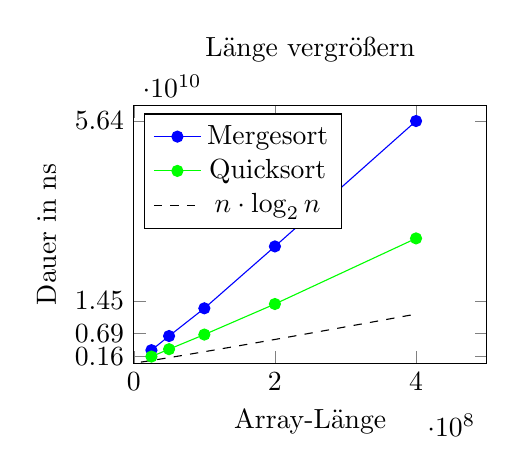
\begin{tikzpicture}
        \begin{axis}[
                title style={yshift=1.5ex},
                width=0.5\textwidth,
                height=0.4\textwidth,
                xlabel={Array-Länge},
                ylabel={Dauer in ns},
                title={Länge vergrößern},
                xmin=0, xmax=5 * 10^8,
                ymin=0*10^6, ymax=6*10^10,
                grid style=dashed,
                legend pos=north west,
                ytick={1609541400,6854920900,14495472700,56441153000},
                % xtick={2^21,2^23,2^24,2^25},
                % xticklabels={$2^{21}$, $2^{23}$, $2^{24}$, $2^{25}$},
                % scaled x ticks=false,
                % scaled y ticks=false,
            ]
            \MergesortMesswerte
            \QuicksortMesswerte
            % n*log2(n)
            \addplot[black, dashed,domain=1e7:4e8, samples=100] {x*log2(x)};
            \addlegendentry{$n \cdot \log_2 n$}
            % % n
            % \addplot[red, dashed,domain=1e7:4e8, samples=100] {x};
            % \addlegendentry{$n$}
            % % log2(n)
            % \addplot[green, domain=1e7:4e8, samples=100] {log2(x)};
            % \addlegendentry{$\log_2 n$}
        \end{axis}
    \end{tikzpicture}%
}

\newcommand{\GrundlegendeLaufzeitenAbhaengigVonDerArraygroesseDiagrammB}{%
    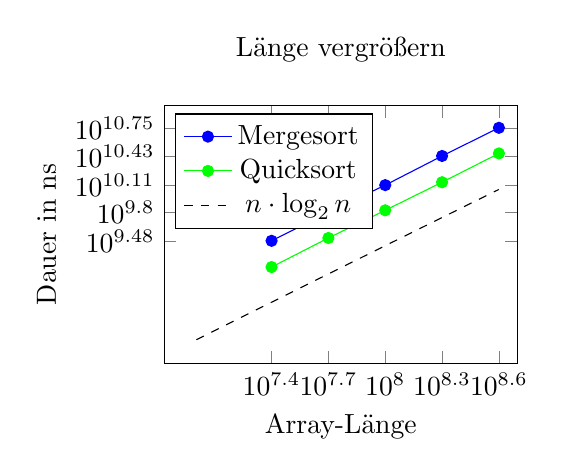
\begin{tikzpicture}
        \begin{axis}[
                title style={yshift=1.5ex},
                width=0.5\textwidth,
                height=0.4\textwidth,
                xlabel={Array-Länge},
                ylabel={Dauer in ns},
                title={Länge vergrößern},
                xmin=0, xmax=5 * 10^8,
                ymin=0*10^6, ymax=1*10^11,
                grid style=dashed,
                legend pos=north west,
                xmode=log,
                log basis x=10,
                xtick=data,
                ymode=log,
                log basis y=10,
                ytick=data,
                % xtick={2^21,2^23,2^24,2^25},
                % xticklabels={$2^{21}$, $2^{23}$, $2^{24}$, $2^{25}$},
                % scaled x ticks=false,
                % scaled y ticks=false,
            ]
            \MergesortMesswerte
            \QuicksortMesswerte
            % n*log2(n)
            \addplot[black, dashed,domain=1e7:4e8, samples=100] {x*log2(x)};
            \addlegendentry{$n \cdot \log_2 n$}
        \end{axis}
    \end{tikzpicture}%
}


% Definiere Variablen
% \newcommand{\Messziel}{Messziel}

% % ----------------------
% % 4. Ergebnisse und Analyse
% % ----------------------
% \newpage
% \chapter{Ergebnisse und Analyse}
% \section{Grundlegende Laufzeiten abhängig von der Arraygröße}
% \subsection{Messziel} % Einleitung
% \subsection{Erwartung}
% \subsection{Diagramm}
% \subsection{Analyse und Interpretation}
% \newpage
% \section{Einfluss des Listentyps} % Listentyps: Zufall, Sortiert, InvertiertSortiert, FastSortiert, Dupliziert
% \subsection{Messziel} % Einleitung
% \subsection{Erwartung}
% \subsection{Diagramm}
% \subsection{Analyse und Interpretation}
% \newpage
% \section{Einfluss der Arraygröße im Detail}
% \subsection{Messziel} % Einleitung
% \subsection{Erwartung}
% \subsection{Diagramm}
% \subsection{Analyse und Interpretation}
% \newpage
% \section{Tiefenbasierte Thread-Erzeugung}
% \subsection{Messziel} % Einleitung
% \subsection{Erwartung}
% \subsection{Diagramm}
% \subsection{Analyse und Interpretation}
% \newpage
% \section{Workerthreads}
% \subsection{Messziel} % Einleitung
% \subsection{Erwartung}
% \subsection{Diagramm}
% \subsection{Analyse und Interpretation}
% \newpage
% \section{Vergleich der Threading-Methoden}
% \subsection{Messziel} % Einleitung
% \subsection{Erwartung}
% \subsection{Diagramm}
% \subsection{Analyse und Interpretation}
% \newpage
% \section{Einfluss des Datentyps der Liste} % Listenart: int, string
% \subsection{Messziel} % Einleitung
% \subsection{Erwartung}
% \subsection{Diagramm}
% \subsection{Analyse und Interpretation}
% % \section{Debug Vs Release}

% % ----------------------
% % 4. Ergebnisse und Analyse
% % ----------------------
% \chapter{Ergebnisse und Analyse}
% \section{Grundlegende Laufzeiten abhängig von der Arraygröße}

% \subsection{Messziel} % Einleitung
\newcommand{\GrundlegendeLaufzeitenAbhaengigVonDerArraygroesseMessziel}{
    Das Messziel besteht darin, die Abhängigkeit des seriellen Algorithmus von der Arraygröße grafisch darzustellen.
    Dadurch können diese Ergebnisse später mit den nicht-seriellen Varianten verglichen werden.
    Gleichzeitig dient dies als einfacher Einstieg in das Thema.
}

% \subsection{Erwartung}
\newcommand{\GrundlegendeLaufzeitenAbhaengigVonDerArraygroesseErwartung}{
    Da die durchschnittliche Laufzeit \(O(n \log n)\) beträgt, erwarte ich eine logarithmische Laufzeiterhöhung bei wachsender Arraygröße.
}
% \subsection{Diagramm}
\newcommand{\GrundlegendeLaufzeitenAbhaengigVonDerArraygroesseDiagramm}{
    \GrundlegendeLaufzeitenAbhaengigVonDerArraygroesseDiagrammA
    \GrundlegendeLaufzeitenAbhaengigVonDerArraygroesseDiagrammB
    \newline
    \GrundlegendeLaufzeitenAbhaengigVonDerArraygroesseDiagrammC
}
% \subsection{Analyse und Interpretation}
\newcommand{\GrundlegendeLaufzeitenAbhaengigVonDerArraygroesseAnalyse}{

}